% Presentación v2: basada en docs/tex/tesis.tex; el centro es la verosimilitud y los datos.
% Compilar: latexmk -pdf presentacion_vero.tex   (reusa figs/ de la presentación v1)
\documentclass[aspectratio=169,11pt]{beamer}
\usepackage[T1]{fontenc}
\usepackage[utf8]{inputenc}
\usepackage[spanish,es-nodecimaldot]{babel}
\usepackage{amsmath,amssymb,booktabs,tikz,graphicx,array}
\usetikzlibrary{arrows.meta,positioning}

\usetheme{default}
\usecolortheme{seahorse}
\definecolor{azul}{RGB}{31,95,191}
\definecolor{rojo}{RGB}{200,60,40}
\definecolor{verde}{RGB}{40,130,70}
\definecolor{gris}{RGB}{90,90,90}
\setbeamercolor{frametitle}{fg=azul}
\setbeamercolor{title}{fg=azul}
\setbeamercolor{structure}{fg=azul}
\setbeamertemplate{navigation symbols}{}
\setbeamertemplate{footline}{\hfill\scriptsize\color{gris}\insertframenumber\,/\,\inserttotalframenumber\hspace{1em}\vspace{0.6em}}
\setbeamertemplate{itemize items}[circle]
\setbeamerfont{frametitle}{size=\large,series=\bfseries}
\setbeamertemplate{blocks}[rounded][shadow=false]
\setbeamercolor{block body}{bg=azul!8,fg=black}
\setbeamercolor{block title}{bg=azul!8,fg=black}

\newcommand{\idea}[1]{\vspace{-0.3em}\begin{block}{}\centering\small #1\end{block}}
\newcommand{\nota}[1]{\par\vfill{\scriptsize\color{gris}#1}}
\newcommand{\obs}[1]{{\color{verde}#1}}
\newcommand{\noobs}[1]{{\color{rojo}#1}}
\tikzset{
  tarjeta/.style={draw=azul!60, rounded corners, fill=azul!6, align=center,
                  text width=#1, inner sep=6pt, font=\small,
                  execute at begin node={\hyphenpenalty=10000\exhyphenpenalty=10000}},
  tarjeta/.default=4.2cm,
  roja/.style={draw=rojo!70, fill=rojo!8},
  verdec/.style={draw=verde!70, fill=verde!8},
  flecha/.style={-{Stealth}, thick, gris},
}

\title{Reparación no observada en un mercado de autos usados}
\subtitle{Cómo se construye la verosimilitud y de qué datos viene}
\author{Rodrigo Antonio Aldrette Salas}
\institute{El Colegio de México \\ Seminario de tesis}
\date{Noviembre 2026}

\begin{document}

\begin{frame}
  \titlepage
\end{frame}

% =====================================================================
\begin{frame}{Pregunta y plan}
  \textbf{Pregunta.} En el mercado de autos usados los hogares compran, venden y
  \textbf{reparan}; la reparación casi nunca se registra (talleres informales).
  \begin{itemize}
    \item ¿Se puede estimar un modelo estructural con una decisión de reparar que el
          econometrista \textbf{no observa}?
    \item ¿Qué se sesga si se estima el modelo de Gillingham et al.\ (2022), que no tiene
          reparación, con datos de una economía donde sí se repara?
  \end{itemize}
  \medskip
  \centering
  \begin{tikzpicture}[node distance=0.4cm]
    \node[tarjeta=3.0cm] (m) {\textbf{1. Modelo}\\[0.2em] Gillingham + desgaste $w$ +
          reparar $r$};
    \node[tarjeta=2.6cm, right=of m, roja] (d) {\textbf{2. Datos}\\[0.2em] qué se ve y
          qué no};
    \node[tarjeta=2.8cm, right=of d, roja] (l) {\textbf{3. Verosimilitud}\\[0.2em] sumar
          sobre lo que no se ve};
    \node[tarjeta=2.4cm, right=of l] (s) {\textbf{4. Monte Carlo}\\[0.2em] ¿funciona?};
    \draw[flecha] (m) -- (d);
    \draw[flecha] (d) -- (l);
    \draw[flecha] (l) -- (s);
  \end{tikzpicture}
  \idea{El corazón de hoy son los pasos 2 y 3 (en rojo).}
\end{frame}

% =====================================================================
\section{Modelo}

\begin{frame}{El modelo en una lámina}
  Equilibrio estacionario del mercado de autos (Rust, 1985; Gillingham et al., 2022).
  Un periodo es un año; dos marcas $j$; dos tipos de hogar $\tau$ (distinta $\mu_\tau$).
  \medskip
  \begin{itemize}
    \item \textbf{Estado del auto:} marca $j$, edad $a$ y \textbf{desgaste} $w$.
    \item \textbf{Decisiones:} mantener, intercambiar o quedarse sin auto; al deshacerse
          del auto, venderlo ($D=0$) o chatarrizarlo ($D=1$); y \noobs{reparar} ($r=1$),
          pagando $R_{ja}$.
    \item \textbf{Precios:} nuevos $\overline P_j$ y chatarra $\underline P_j$ fijos;
          usados $P_{jaw}$ \textbf{endógenos} (vacían el mercado).
    \item \textbf{Utilidad:} $u_\tau(j,a,w)=u_{0,\tau j}+u_{1,\tau j}\,a+u_w\,w$ menos
          $\mu_\tau\times$(gastos netos), con costos de transacción $T_{b,\tau}$, $T_s$.
    \item \textbf{Choques} GEV (logit anidado): probabilidades $\Pi(\cdot)$ en forma
          cerrada.
  \end{itemize}
  \idea{Respecto a Gillingham, lo nuevo es $w$ y $r$: dos autos de la misma marca y edad
  pueden valer distinto, y el dueño puede invertir en el suyo.}
\end{frame}

\begin{frame}{Desgaste y reparación}
  \begin{columns}[c]
    \column{0.55\textwidth}
    \small
    \textbf{Probabilidad de avería} (el auto sale del parque):
    \[
      s(j,a,w)=\Lambda\big(\underbrace{\alpha_{0j}+\alpha_{1j}\,a}_{\text{envejecimiento}}
               +\underbrace{w}_{\text{desgaste}}\big)
    \]
    \textbf{Si sobrevive}, el desgaste evoluciona (Hu \& Xin, 2024):
    \[
      w'=w+\delta_j-\kappa\,r+\eta,\qquad \eta\sim N(0,\sigma_\eta^2)
    \]
    Escribimos $f(w'\mid j,a,w,r)$ para esta densidad.
    \medskip

    \textbf{Reparar} compara costo de hoy y ganancia de mañana:
    \[
      \Pi(r=1\mid h)=\Lambda\!\left(\frac{v_1(h)-v_0(h)}{\sigma_r}\right),
    \]
    con $v_1$ que incluye el costo $-\mu_\tau R_{ja}$.
    \column{0.43\textwidth}
    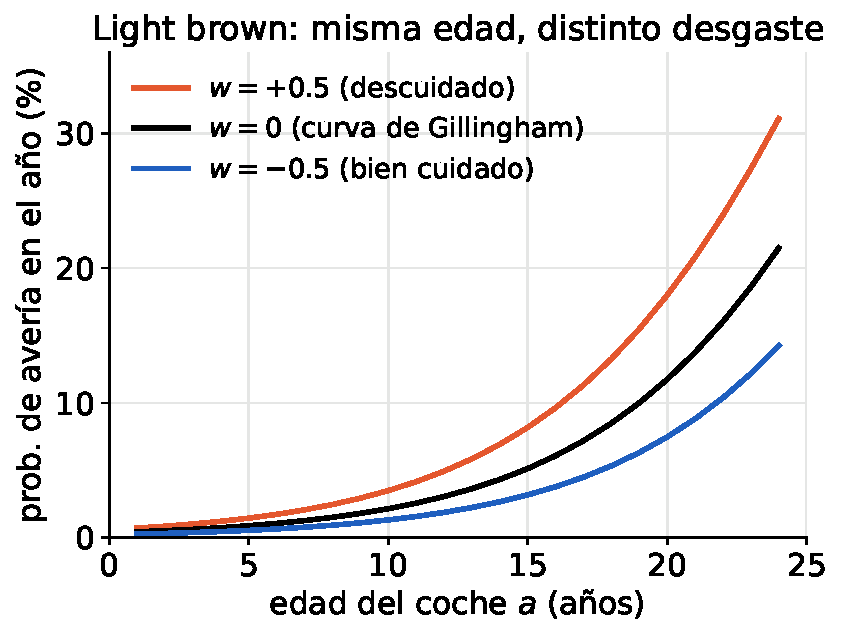
\includegraphics[width=\linewidth]{figs/fig_desgaste.pdf}
    \par\smallskip
    {\scriptsize Los nuevos nacen con $w=0$. La reparación se aprecia hasta el año
    siguiente: la avería de este año depende del $w$ con el que empezó.}
  \end{columns}
\end{frame}

\begin{frame}{Un año en la economía y el equilibrio}
  \centering
  \begin{tikzpicture}[node distance=0.5cm and 0.3cm,
      caja/.style={draw=azul!70, rounded corners, fill=azul!6, align=center,
                   font=\footnotesize, minimum height=1.2cm, text width=2.3cm}]
    \node[caja] (x) {Inicio\\$x=(j,a,w)$};
    \node[caja, right=of x] (c) {Intercambio\\mantener / cambiar\\/ sin auto};
    \node[caja, right=of c, fill=rojo!8, draw=rojo!70] (r) {Reparar\\$r\in\{0,1\}$};
    \node[caja, right=of r] (f) {Uso\\avería con\\prob.\ $s(h)$};
    \node[caja, right=of f, text width=2.6cm] (w) {Si sobrevive:\\$a'=a+1$\\$w'=w+\delta_j-\kappa r+\eta$};
    \draw[flecha] (x) -- (c);
    \draw[flecha] (c) -- node[above, font=\scriptsize]{$h$} (r);
    \draw[flecha] (r) -- (f);
    \draw[flecha] (f) -- (w);
    \draw[flecha] (w.south) -- ++(0,-0.5) -| node[pos=0.25, below, font=\scriptsize]{siguiente año} (x.south);
    \node[above=0.1cm of c, font=\scriptsize, gris] {$\Omega(P,R)$};
    \node[above=0.1cm of f, font=\scriptsize, gris] {$Q$};
    \node[above=0.1cm of w, font=\scriptsize, gris] {$A(P,R)$};
  \end{tikzpicture}
  \vspace{0.6em}
  \begin{itemize}
    \item \textbf{Equilibrio} en cada mercado $m$:\quad
          $q_{m\tau}\,\Omega_\tau\,Q\,A_\tau=q_{m\tau}$ (distribución estacionaria)\quad y\quad
          $ED(P_m,q_m)=0$ (vaciado).
    \item \textbf{Regímenes:} $M=3$ mercados idénticos salvo el precio de reparar,
          $R_m=R\,e^{\zeta_m}$, $\zeta_m\in\{-0.3,0,0.3\}$. Cada uno en su propio equilibrio
          $\big(P_m(\theta),q_m(\theta)\big)$.
  \end{itemize}
  \idea{Para estimar solo necesitamos dos cosas del equilibrio: las probabilidades $\Pi$ y
  los precios $P_m(\theta)$ que entran en ellas.}
\end{frame}

% =====================================================================
\section{Datos}

\begin{frame}{¿De qué datos viene la verosimilitud?}
  \small Un panel de hogares como el registro danés de Gillingham, más dos variables:
  el estado del auto ($w$) y el régimen de precios de reparar ($R_m$).
  \begin{center}\footnotesize
  \begin{tabular}{lll}
    \toprule
    & Variable & Comentario\\
    \midrule
    \obs{Se observa} & tipo $\tau$ y mercado $m$ & heterogeneidad persistente\\
    & tenencia $\delta_t$: $(j,a,w)$, nuevo $(j,0)$ o $\emptyset$ & después del intercambio\\
    & qué pasó con el auto, $e_{t+1}\in\{K,D{=}0,D{=}1\}$ & mantener, vender o chatarrizar\\
    & desgaste $w'$ del auto si sigue circulando & si se mantuvo o se vendió\\
    & la nueva tenencia $\delta_{t+1}$ & qué compró (con su $w$)\\
    & precios $\overline P_j$, $\underline P_j$, $R_m$ & datos\\
    \midrule
    \noobs{No se observa} & reparación $r$ & nunca\\
    & motivo de la chatarrización & ¿avería o decisión?\\
    & $w'$ de un auto chatarrizado & ya no circula\\
    & precios de los usados $P_{jaw}$ & salen del modelo: $P_m(\theta)$\\
    \bottomrule
  \end{tabular}
  \end{center}
  \idea{Una observación es una \textbf{transición} de un hogar de un año al siguiente:
  $\big(\delta_t,\;e_{t+1},\;w'_{t+1},\;\delta_{t+1}\big)$.}
\end{frame}

\begin{frame}{Una observación: qué pasa entre $\delta_t$ y $\delta_{t+1}$}
  \centering
  \begin{tikzpicture}[
      n/.style={draw=azul!60, rounded corners, fill=azul!6, align=center,
                font=\scriptsize, text width=1.9cm, inner sep=3pt, minimum height=0.9cm},
      e/.style={-{Stealth}, gris, thick},
      lab/.style={font=\scriptsize, inner sep=1.5pt}]
    \node[n, verdec] (h) at (0,0) {$\delta_t=(j,a,w)$\\ \obs{se observa}};
    \node[n, roja] (acc) at (3.0,1.5) {avería:\\terminal $(j,\bar a)$};
    \node[n] (sob) at (3.0,-0.8) {sobrevive};
    \node[n, roja] (r1) at (6.0,0.1) {reparó};
    \node[n, roja] (r0) at (6.0,-1.7) {no reparó};
    \node[n, verdec] (w) at (9.0,-0.8) {$(j,a{+}1,w')$\\ \obs{$w'$ si circula}};
    \node[n, verdec, text width=2.3cm] (d) at (12.3,0.4) {intercambio:\\ \obs{$e_{t+1}$ y $\delta_{t+1}$}};
    \draw[e] (h) -- node[lab, above left]{$s$} (acc);
    \draw[e] (h) -- node[lab, below left]{$1-s$} (sob);
    \draw[e, rojo, dashed] (sob) -- node[lab, above left]{$\Pi(r{=}1\mid h)$} (r1);
    \draw[e, rojo, dashed] (sob) -- node[lab, below left]{$\Pi(r{=}0\mid h)$} (r0);
    \draw[e] (r1) -- node[lab, above right]{$f(w'\mid r{=}1)$} (w);
    \draw[e] (r0) -- node[lab, below right]{$f(w'\mid r{=}0)$} (w);
    \draw[e] (w) -- node[lab, below right]{$\Pi(\cdot\mid j,a{+}1,w')$} (d);
    \draw[e] (acc) -- node[lab, above, sloped, pos=0.45]{$\Pi(\cdot\mid j,\bar a)$, chatarra obligatoria} (d);
    \node[font=\scriptsize, gris] at (1.5,-2.5) {matriz $Q$};
    \node[font=\scriptsize, gris] at (7.5,-2.5) {matriz $A(P,R)$};
    \node[font=\scriptsize, gris] at (12.3,-2.5) {matriz $\Omega(P,R)$};
  \end{tikzpicture}
  \par\smallskip
  \raggedright
  {\small Como observamos tenencias post-intercambio,
  $\;\Pr(\delta_{t+1}\mid\delta_t)=\big[Q\,A(P,R)\,\Omega(P,R)\big]_{\delta_t,\delta_{t+1}}$.}
  \idea{Regla de la verosimilitud: lo que está en \noobs{rojo} no se ve, así que se
  \textbf{suma sobre todos sus caminos}.}
\end{frame}

% =====================================================================
\section{Verosimilitud}

\begin{frame}{Pieza 1: la reparación no observada es una mezcla}
  Si el auto sobrevive vemos $w'$, pero no si se reparó. La probabilidad de llegar a
  $w'$ suma los dos caminos:
  \vspace{-0.4em}
  \[
    Z(w'\mid h)=\Pi(r{=}1\mid h,P_m,R_m)\,f(w'\mid h,r{=}1)
      +\Pi(r{=}0\mid h,P_m,R_m)\,f(w'\mid h,r{=}0)
  \]
  \vspace{-1.2em}
  \begin{columns}[c]
    \column{0.40\textwidth}
    \begin{itemize}\small
      \item Es la ec.\ (6.4) de Hu \& Xin (2024): \emph{observabilidad parcial}.
      \item $f$ es la misma en todos los mercados; lo que cambia con $R_m$ son los
            \textbf{pesos} $\Pi(r\mid h)$.
      \item Con mercados distintos se separan las dos campanas.
    \end{itemize}
    \column{0.58\textwidth}
    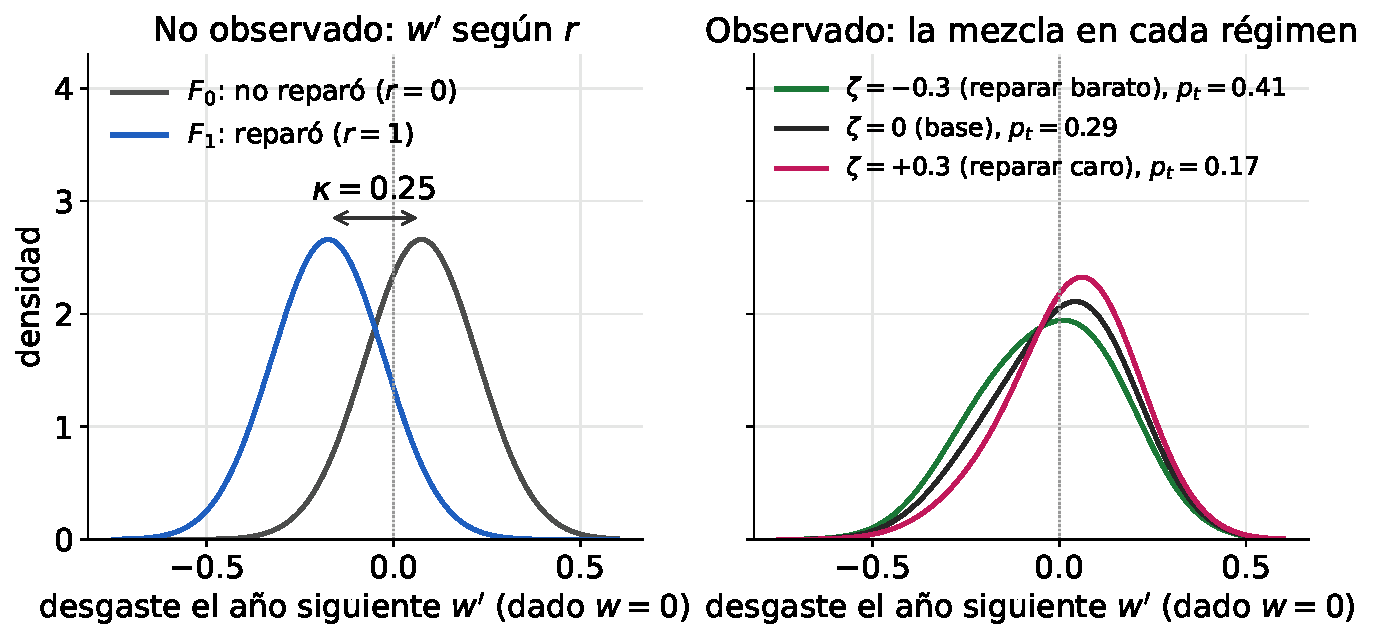
\includegraphics[width=\linewidth]{figs/fig_mezcla.pdf}
  \end{columns}
  \idea{El precio de reparar es la variable excluida: mueve la decisión, no la física del
  auto (Supuesto 7 de Hu \& Xin).}
\end{frame}

\begin{frame}{Pieza 2: las contribuciones de cada observación}
  Partiendo de $\delta_t=(j,a,w)$, con $s=s(j,a,w)$:
  \vspace{-0.6em}
  \begin{center}\small
  \renewcommand{\arraystretch}{1.3}
  \begin{tabular}{l>{$}l<{$}}
    \toprule
    Lo observado & \text{contribución } l\\
    \midrule
    Mantuvo ($w'$ visto) &
      (1-s)\;\noobs{Z(w'\mid j,a,w)}\;\Pi(K\mid j,a{+}1,w')\\
    Vendió ($D{=}0$, $w'$ visto) &
      (1-s)\;\noobs{Z(w'\mid j,a,w)}\;\Pi(\delta_{t+1},D{=}0\mid j,a{+}1,w')\\
    Chatarrizó ($D{=}1$) &
      \underbrace{s\,\Pi(\delta_{t+1}\mid j,\bar a)}_{\text{avería}}\\
    & {}+\underbrace{(1-s)\noobs{\textstyle\sum_{w'}Z(w'\mid j,a,w)}\,
        \Pi(\delta_{t+1},D{=}1\mid j,a{+}1,w')}_{\text{chatarreo voluntario}}\\
    Sin auto en $t$ & \Pi(\delta_{t+1}\mid\emptyset)\\
    \bottomrule
  \end{tabular}
  \end{center}
  \begin{itemize}\small
    \item $\delta_{t+1}$ puede ser un usado $(i,b,y)$, un nuevo $(i,0)$ o $\emptyset$.
    \item Desde un nuevo $(j,0)$: lo mismo con $a=0$, $w=0$ y $Z=f(\cdot\mid j,0,0,r{=}0)$.
  \end{itemize}
  \idea{Dos sumas sobre lo no observado: sobre $r$ (dentro de $Z$) y, al chatarrizar,
  sobre avería contra decisión y sobre el $w'$ que no vimos.}
\end{frame}

\begin{frame}{Un ejemplo: el hogar que chatarriza}
  Un hogar con un LB de 10 años y $w=0.2$; al año siguiente lo vemos con un nuevo HB y
  sabemos que el LB se chatarrizó. ¿Por qué?
  \medskip
  \centering
  \begin{tikzpicture}[node distance=0.6cm]
    \node[tarjeta=5.4cm, roja, minimum height=2.6cm] (a) {\textbf{Camino 1: avería}\\[0.3em]
      prob.\ $s(\text{LB},10,0.2)$\\[0.2em] luego, desde el terminal,\\ compra un HB nuevo:
      $\Pi(\text{HB},0\mid \text{LB},\bar a)$};
    \node[tarjeta=6.0cm, roja, minimum height=2.6cm, right=of a] (b) {\textbf{Camino 2:
      sobrevivió y decidió chatarrizar}\\[0.3em] prob.\ $1-s$, llega a algún $w'$ con
      $Z(w'\mid\cdot)$\\[0.2em] (reparó o no) y elige ``chatarrizar y comprar HB nuevo'':\\
      $\Pi(\text{HB},0,D{=}1\mid \text{LB},11,w')$};
  \end{tikzpicture}
  \par\medskip
  \raggedright
  \[
    l=s\cdot\Pi(\text{HB},0\mid\text{LB},\bar a)\;+\;(1-s)\sum_{w'}Z(w'\mid\text{LB},10,0.2)\,
      \Pi(\text{HB},0,D{=}1\mid\text{LB},11,w')
  \]
  \idea{Aquí está toda la dificultad: tres cosas no observadas (avería, $r$, $w'$) se
  integran en una sola probabilidad que sí se puede calcular.}
\end{frame}

\begin{frame}{Pieza 3: la verosimilitud por celdas}
  Como los estados son discretos y los tipos se observan, dos transiciones con lo mismo
  observado tienen la misma contribución. Una \textbf{celda} es
  \[
    c=\big(m,\;\tau,\;\delta_t,\;e_{t+1},\;w'_{t+1},\;\delta_{t+1}\big),
    \qquad N_c=\#\text{ transiciones en }c
  \]
  \vspace{-0.8em}
  \[
    \boxed{\;LL(\theta)=\sum_{m=1}^{M}\sum_{g}\sum_{t=1}^{T-1}\log l_{gmt}
      =\sum_{c}N_c\,\log l_c\big(\theta,P_{m_c}(\theta)\big)\;}
  \]
  \begin{center}\small
  \begin{tabular}{cccccc|r}
    \toprule
    $m$ & $\tau$ & $\delta_t$ & $e_{t+1}$ & $w'$ & $\delta_{t+1}$ & $N_c$\\
    \midrule
    base & pareja & (LB, 10, 0.2) & $K$ & 0.25 & (LB, 11, 0.25) & 14\\
    base & pareja & (LB, 10, 0.2) & $D{=}0$ & 0.10 & (HB, 3, 0.0) & 2\\
    barato & soltero & (LB, 10, 0.2) & $D{=}1$ & --- & (HB, 0) & 1\\
    \bottomrule
  \end{tabular}
  \end{center}
  {\small Agrupar es exacto, no una aproximación: solo cambia el costo de evaluar $LL$,
  que depende del número de celdas y no del de hogares. Condicionamos en la primera
  tenencia, como Gillingham.}
  \nota{Los números de la tabla son ilustrativos.}
\end{frame}

\begin{frame}{Pieza 4: dónde entra el equilibrio (punto fijo anidado)}
  \centering
  \begin{tikzpicture}[node distance=0.35cm and 0.35cm,
      caja/.style={draw=azul!70, rounded corners, fill=azul!6, align=center,
                   font=\footnotesize, minimum height=1.4cm, text width=2.0cm}]
    \node[caja, text width=1.9cm] (t) {$\theta$\\ (26 parám.)};
    \node[caja, right=of t, text width=3.4cm] (e) {Para cada mercado $m$:\\ Bellman
          $EV_\tau=\Gamma(EV_\tau;P,R_m)$\\ y vaciado $ED(P_m)=0$};
    \node[caja, right=of e] (p) {$\Pi_\tau(\cdot)$, $Z$, $s$\\ a precios $P_m(\theta)$};
    \node[caja, right=of p] (l) {$l_c$ en cada celda};
    \node[caja, right=of l, text width=1.4cm] (L) {$LL(\theta)$};
    \draw[flecha] (t) -- (e);
    \draw[flecha] (e) -- (p);
    \draw[flecha] (p) -- (l);
    \draw[flecha] (l) -- (L);
    \draw[flecha] (L.south) -- ++(0,-0.6) -| node[pos=0.25, below, font=\scriptsize]
      {optimizador: nuevo $\theta$} (t.south);
  \end{tikzpicture}
  \vspace{0.6em}
  \begin{itemize}
    \item Como en Rust (1987) y Gillingham: cada evaluación de $LL$ resuelve los equilibrios.
    \item \textbf{Sin instrumentos}, a diferencia de BLP: no hay características no
          observadas de los autos y los precios de usados no se usan como dato, se
          sustituyen por $P_m(\theta)$.
    \item $\hat\theta=\arg\max_\theta LL(\theta)$. Todos los mercados comparten $\theta$.
  \end{itemize}
\end{frame}

\begin{frame}{¿Qué dato identifica qué parámetro? (intuición)}
  \begin{center}\small
  \renewcommand{\arraystretch}{1.25}
  \begin{tabular}{p{4.2cm}p{8.6cm}}
    \toprule
    Parámetros & Variación en los datos\\
    \midrule
    $\delta_j,\ \kappa,\ \sigma_\eta$ (desgaste) & la forma de la distribución de $w'$
      dado $w$: una mezcla de dos normales separadas por $\kappa$\\
    $\Pi(r\mid h)$, $\sigma_r$ (reparar) & cómo cambian los pesos de la mezcla entre
      mercados con distinto $R_m$\\
    $\alpha_{0j},\ \alpha_{1j}$ (avería) & salidas del parque por edad, con $w$ fijo
      (envejecimiento contra desgaste)\\
    $u_{0},\ u_{1},\ u_w,\ \mu_\tau$ & mantener contra cambiar según $(j,a,w)$, y qué
      autos se compran; $\overline P_j$, $\underline P_j$, $R_m$ fijan la escala en dinero\\
    $T_{b,\tau},\ T^{\emptyset}_{b,\tau},\ T_s,\ \sigma_D$ & frecuencia de transacciones
      y de vender contra chatarrizar\\
    \bottomrule
  \end{tabular}
  \end{center}
  \begin{itemize}\small
    \item Sin precios de usados, $T_b$ y $T_s$ solo se separan con \textbf{dos tipos de
          hogar con $\mu_\tau$ distinta}: subir $T_b$, bajar $T_s$ y bajar todos los
          precios en lo mismo deja igual cada transacción.
  \end{itemize}
  \idea{Sin variación en $R_m$, la mezcla no separa ``reparó'' de ``tuvo suerte con
  $\eta$''.}
\end{frame}

% =====================================================================
\section{Monte Carlo}

\begin{frame}{Monte Carlo: los datos se simulan y luego se borran columnas}
  \centering
  \begin{tikzpicture}[node distance=0.35cm]
    \node[tarjeta=2.8cm, minimum height=2.1cm] (p1) {\textbf{1. Equilibrio}\\ con
          $\theta$ verdadero en los 3 mercados};
    \node[tarjeta=2.8cm, minimum height=2.1cm, right=of p1] (p2) {\textbf{2. Panel}\\
          10{,}000 hogares por mercado, 4 años};
    \node[tarjeta=2.8cm, minimum height=2.1cm, right=of p2] (p3) {\textbf{3. Borrar}\\
          lo que no se ve según el diseño};
    \node[tarjeta=2.8cm, minimum height=2.1cm, right=of p3] (p4) {\textbf{4. Estimar}\\
          y repetir con paneles nuevos};
    \draw[flecha] (p1) -- (p2);
    \draw[flecha] (p2) -- (p3);
    \draw[flecha] (p3) -- (p4);
  \end{tikzpicture}
  \par\medskip
  {\small $N(T-1)M=90{,}000$ transiciones por réplica. Parámetros comunes de Gillingham
  et al.\ (2022, ap.\ F); desgaste y reparación calibrados.}
  \begin{center}\footnotesize
  \begin{tabular}{llcc}
    \toprule
    Estimador & Verosimilitud & Ve $r$ & Ve motivo de salida\\
    \midrule
    Diseño 1 & sin mezclas (cota superior) & sí & sí\\
    Diseño 2 & mezcla sobre $r$ ($Z$) & no & sí\\
    Diseño 3 & la de estas láminas (datos reales) & no & no\\
    Gillingham parcial / completa & sin $w$ ni $r$ & --- & no / sí\\
    \bottomrule
  \end{tabular}
  \end{center}
  \idea{Mismo panel para todos: las diferencias entre diseños vienen solo de la
  información, no de la muestra.}
\end{frame}

\begin{frame}{Qué buscamos medir}
  \begin{enumerate}
    \item \textbf{¿El estimador funciona?} El diseño 3 recupera $\theta$ y la tasa de
          reparación, con errores estándar correctos, aun sin ver $r$.
    \item \textbf{¿Cuánto cuesta no observar?}
          \begin{itemize}
            \item Diseño 1 contra 2: el costo de no ver la reparación.
            \item Diseño 2 contra 3: el costo adicional de no distinguir avería de
                  chatarreo.
          \end{itemize}
    \item \textbf{¿Cuánto se sesga Gillingham?} Estimado sobre estos datos converge a
          valores pseudo-verdaderos; la distancia a la verdad es el sesgo de ignorar la
          reparación (en parámetros y en los precios de equilibrio que implica).
  \end{enumerate}
  \idea{La corrida preliminar sugiere: diseños sin sesgo; Gillingham con $\mu$ muy por
  debajo. La corrida final con esta especificación está pendiente.}
\end{frame}

% =====================================================================
\begin{frame}{Resumen}
  \vspace{0.5em}
  \centering
  \begin{tikzpicture}[node distance=0.45cm]
    \node[tarjeta=3.9cm, minimum height=3.4cm] (a) {\textbf{Datos}\\[0.5em] transiciones
          de tenencia, como Gillingham, más $w$ y el régimen $R_m$; sin $r$, sin motivo de
          salida, sin precios de usados};
    \node[tarjeta=3.9cm, minimum height=3.4cm, roja, right=of a] (b) {\textbf{Verosimilitud}\\[0.5em]
          suma sobre lo no observado: $Z$ mezcla sobre $r$; avería contra chatarreo y
          el $w'$ no visto};
    \node[tarjeta=3.9cm, minimum height=3.4cm, right=of b] (c) {\textbf{Identificación}\\[0.5em]
          la variación en el precio de reparar mueve los pesos de la mezcla, no la
          física (Hu \& Xin)};
  \end{tikzpicture}
  \vspace{0.8em}
  \idea{$\displaystyle LL(\theta)=\sum_c N_c\log l_c\big(\theta,P_{m_c}(\theta)\big)$: una
  sola verosimilitud, un solo paso, con el equilibrio adentro.}
\end{frame}

\begin{frame}
  \centering\Large Gracias\\[1em]
  \normalsize Rodrigo Antonio Aldrette Salas
\end{frame}

% =====================================================================
\appendix

\begin{frame}{Apéndice: árbol de decisiones de un dueño}
  \centering
  \begin{tikzpicture}[level distance=1.5cm,
      level 1/.style={sibling distance=5.2cm},
      level 2/.style={sibling distance=2.5cm},
      every node/.style={draw=azul!60, rounded corners, fill=azul!5, font=\small, align=center},
      edge from parent/.style={draw, gris, -{Stealth}}]
    \node {Dueño de $x=(j,a,w)$}
      child { node {Deshacerse}
        child { node {Vender $D{=}0$} }
        child { node {Chatarrizar $D{=}1$} } }
      child { node {Mantener}
        child { node[fill=rojo!8, draw=rojo!60] {Reparar} }
        child { node[fill=rojo!8, draw=rojo!60] {No reparar} } }
      child { node {Intercambiar}
        child { node {$D\in\{0,1\}$\\ y comprar $h$} }
        child { node[fill=rojo!8, draw=rojo!60] {Reparar o no\\ $h$} } };
  \end{tikzpicture}
  \begin{itemize}\small
    \item Rojo: no se observa. Los nuevos y los de edad $\bar a-1$ no se reparan.
    \item La probabilidad de reparar es la misma si el hogar mantuvo o compró el auto:
          por eso la mezcla $Z$ depende solo de la tenencia $h$.
  \end{itemize}
\end{frame}

\begin{frame}{Apéndice: supuestos de Hu \& Xin (2024) en el modelo}
  \begin{itemize}
    \item \textbf{Error aditivo} (Sup.\ 2): $w'=m(j,r,w)+\eta$, $\eta$ independiente de
          $r$; por eso $w$ está en log-momios.
    \item \textbf{Transición estable} (Sup.\ 1): $f(w'\mid j,a,w,r)$ no depende del
          mercado ni del tiempo.
    \item \textbf{Variable excluida} (Sup.\ 7): $R_m$ mueve $\Pi(r\mid\cdot)$, no $f$. En
          horizonte infinito hace el papel que en horizonte finito hace el tiempo.
    \item \textbf{Observabilidad parcial} (sec.\ 6.3): se ve mantener/intercambiar, no
          reparar.
    \item Ellos identifican $f$ de forma no paramétrica en un primer paso; aquí $f$ es
          paramétrica y todo se estima en un paso.
    \item Discretización: $W=71$ puntos en $[-3,2.25]$, paso $\sigma_\eta/2$; en los bordes
          $E[\eta\mid w]\neq0$, por eso se pide masa $<0.5\%$ en los extremos.
  \end{itemize}
\end{frame}

\begin{frame}{Apéndice: parámetros del Monte Carlo}
  \begin{columns}[T]
    \column{0.5\textwidth}
    \scriptsize
    \begin{tabular}{@{}lll@{}}
      \toprule
      \multicolumn{3}{@{}l}{\emph{De Gillingham et al.\ (2022, ap.\ F)}}\\
      $\overline P_j$ & 142.3 / 275.8 & LB / HB, miles DKK\\
      $\alpha_{0j},\alpha_{1j}$ & Tabla 4 & avería\\
      $\mu_\tau$ & 0.113 / 0.094 & pareja / soltero pobres\\
      $u_{0},u_{1}$ & Tablas 8--9 & \\
      $T_{b,\tau},T^{\emptyset}_{b,\tau}$ & Tabla 10 & \\
      $T_s,\sigma_D$ & 0.91, 0.35 & Tabla 5\\
      \bottomrule
    \end{tabular}
    \column{0.46\textwidth}
    \scriptsize
    \begin{tabular}{@{}lll@{}}
      \toprule
      \multicolumn{3}{@{}l}{\emph{Calibración propia}}\\
      $\kappa$ & 0.25 & efecto de reparar\\
      $\sigma_\eta$ & 0.15 & choque al desgaste\\
      $\delta_j$ & $\kappa\bar p=0.075$ & desgaste anual\\
      $u_w$ & $-0.2$ & molestia del desgaste\\
      $\sigma_r$ & 0.3 & escala de reparar\\
      $\beta$, $\bar a$, $\underline P_j$ & 0.95, 25, 2 & \\
      \bottomrule
    \end{tabular}
  \end{columns}
  \medskip
  \centering
  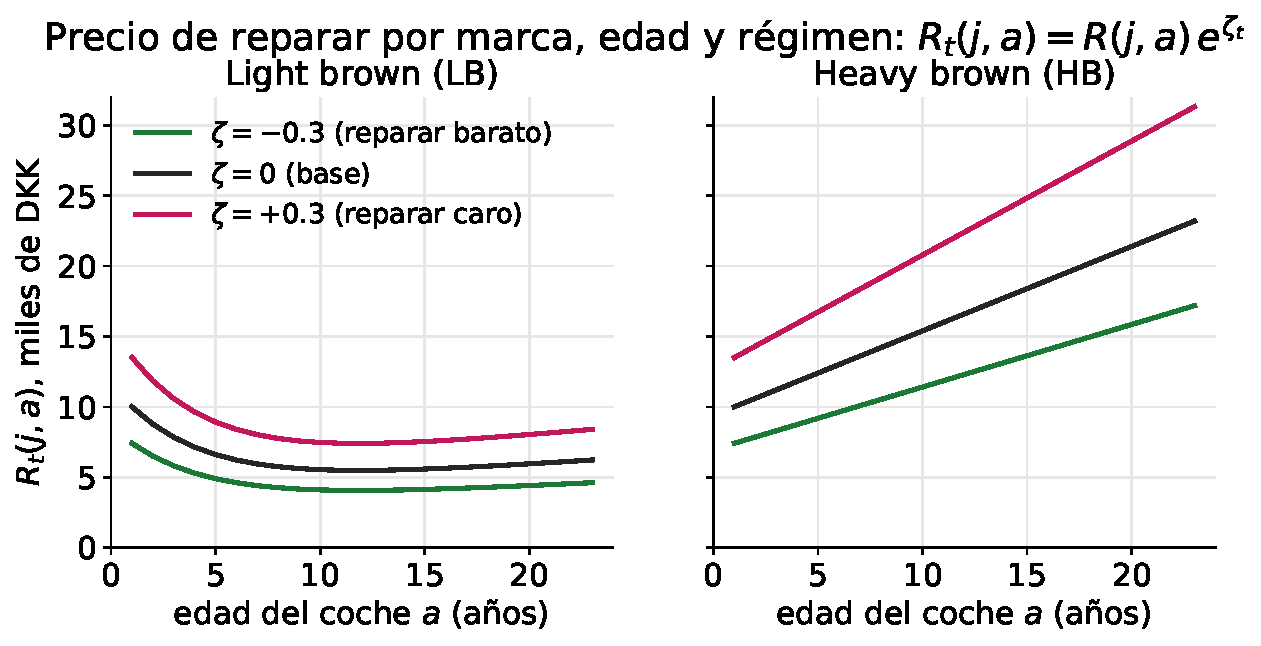
\includegraphics[width=0.62\linewidth]{figs/fig_R.pdf}
\end{frame}

\end{document}
